\documentclass[]{article}
\usepackage[T1]{fontenc}
\usepackage[utf8]{inputenc}
\usepackage[italian]{babel}
\usepackage{amsmath,amssymb}
\usepackage{graphicx}
\newcommand{\numberset}{\mathbb}
\newcommand{\N}{\numberset{N}}
\newcommand{\R}{\numberset{R}}
\usepackage[a4paper, total={6in, 8in}]{geometry}
\usepackage{mathrsfs,amsmath} 

\begin{document}

\begin{center}
\begin{Large}
\textbf{Formulario Di Segnali}
\end{Large}
\end{center}



\textit{\textbf{ 1. Sistemi lineari tempo invarianti}}
\begin{enumerate}
\item \textit{1. Proprietà delle funzioni delta}
\\
\begin{enumerate}
\item
Proprietà dell' area

\[ \sum_{k=-\infty}^{\infty} \delta_{n-k} =1 \]
\begin{equation}
\int_{- \infty}^{\infty} \delta(t) dt =1
\end{equation}
\item \textit{Proprietà della singola componente}
\[ x_n \delta_{n-k}= x_k \delta_{n-k} \]

\begin{equation}
x(t) \delta(t- \tau)= x(\tau) \delta(t- \tau)
\end{equation}

\end{enumerate}


\item \textit{Scomposizione di un segnale mediante funzione delta}
\\
Nel caso di segnali discreti, si può far uso della delta di Kronecker
\begin{equation}
x_n = \sum_{k=-\infty}^{\infty} x_k \delta_{n-k}
\end{equation}
\\
Per i segnali tempo continui  si fa uso della delta di Dirac

\begin{equation}
x(t) = \int_{- \infty}^{\infty} x( \tau) \delta(t- \tau) d \tau
\end{equation}

\item \textit{Sistemi lineari }
\\
Sia $L$ un' applicazione lineare sullo spazio delle funzioni, allora 
\begin{equation}
L(x_1(t) + \alpha x_2(t))=  L(x_1(t)) + \alpha L(x_2(t))
\end{equation}

\item \textit{Sistemi tempo invarianti}
\\
Un sistema tempo invariante è un sistema che lascia passare i ritardi

\begin{equation}
x(t- \tau) \to L \to y(t- \tau) \ \ \ \ \forall \tau \in \R
\end{equation}

\item \textit{Risposta di un sistema LTI ad un ingresso $x(t)$}
\\
Sia $h(t)$ la risposta del sistema all' impulso $\delta(t)$, allora 

\begin{equation}
y(t) = x(t)*y(t) = \int_{- \infty}^{\infty} x(t) h(t- \tau) d \tau
\end{equation}

\item \textit{Proprietà della convoluzione}
\begin{enumerate}
\item Proprietà associativa
\\
Permette le aggregazioni o le disgregazioni di blocchi in serie tra di loro
\begin{equation}
x(t)*[h(t)*g(t)]=[x(t)*h(t)]*g(t)
\end{equation}

\item Proprietà distributiva
\\
Permette le aggregazioni o le disgregazioni di blocchi in parallelo tra di loro

\begin{equation}
x(t)*[h(t)+g(t)]=x(t)*h(t)+x(t)*g(t)
\end{equation}

\item Proprietà commutativa
\\
Permette di concludere che il ruolo di \textit{segnale in ingresso } e \textit{risposta all' impulso di un sistema LTI} sono interscambiabili
\begin{equation}
x(t)*h(t)=h(t)*x(t)
\end{equation}
\\
Come conseguenza vi è la \textbf{\textit{proprietà del ritardo}} che vale solo per sistemi LTI, cioè se $y(t)=x(t)*h(t)$, allora vale che
\begin{equation}
x(t-t_x)*h(t-t_h)= y(t-t_x-t_h)
\end{equation}

 \textbf{TIPO DI ESERCIZIO: CONVOLUZIONE DI RETTANGOLI} \\
Calcolare
\[ y(t)=\left[ rect \left( \frac{t+ \frac{T}{2}}{T} \right) -rect \left( \frac{t- \frac{T}{2}}{T}\right) \right] * 2rect \left( \frac{t- \frac{3T}{2}}{3T}\right) \]
Per procedere conviene sempre scrivere i rettangoli come \textit{generiche funzioni}. Ad esempio assegniamo
\[ f(t)= rect \left( \frac{t}{T} \right) \Rightarrow f \left( t+ \frac{T}{2}\right)= rect \left( \frac{t+ \frac{T}{2}}{T} \right) \ \ \ \  f \left( t- \frac{T}{2}\right)= rect \left( \frac{t- \frac{T}{2}}{T}\right) \]

\[g(t)= rect \left( \frac{t}{3T}\right) \Rightarrow g\left( t- \frac{3T}{2}\right)= rect \left( \frac{t- \frac{3T}{2}}{3T}\right)\]
Pertanto il nostro problema iniziale può essere scritto come
\[y(t)= \left[  f \left( t+ \frac{T}{2}\right) - f \left( t- \frac{T}{2}\right)  \right] * 2g\left( t- \frac{3T}{2}\right)   \]

Facendo uso della proprietà distributiva, posso moltiplicare la $g$ all' interno della parentesi

\[ y(t)=2 \left[  f \left( t+ \frac{T}{2}\right)*g\left( t- \frac{3T}{2}\right) - f \left( t- \frac{T}{2}\right)*g\left( t- \frac{3T}{2}\right)  \right]\]
Il \textit{passaggio chiave }, arrivati a questo punto, è definire una funzione
\[ z(t)=f(t)*g(t)\]
in modo da poter utilizzare la proprietà del ritardo e poter riscrivere 

\[y(t)= 2 \left[ z(t-T) - z( t-2T) \right] \]

Plottiamo la $z(t)$ e i suoi ritardi e l'esercizio è finito. Il grosso dell' esercizio era nel ricondursi ad una forma più semplice usando \textit{la proprietà del ritardo}.
\\
Può essere utile ricordare il seguente disegno che rappresenta la convoluzione tra due segnali rettangolari

\begin{center}
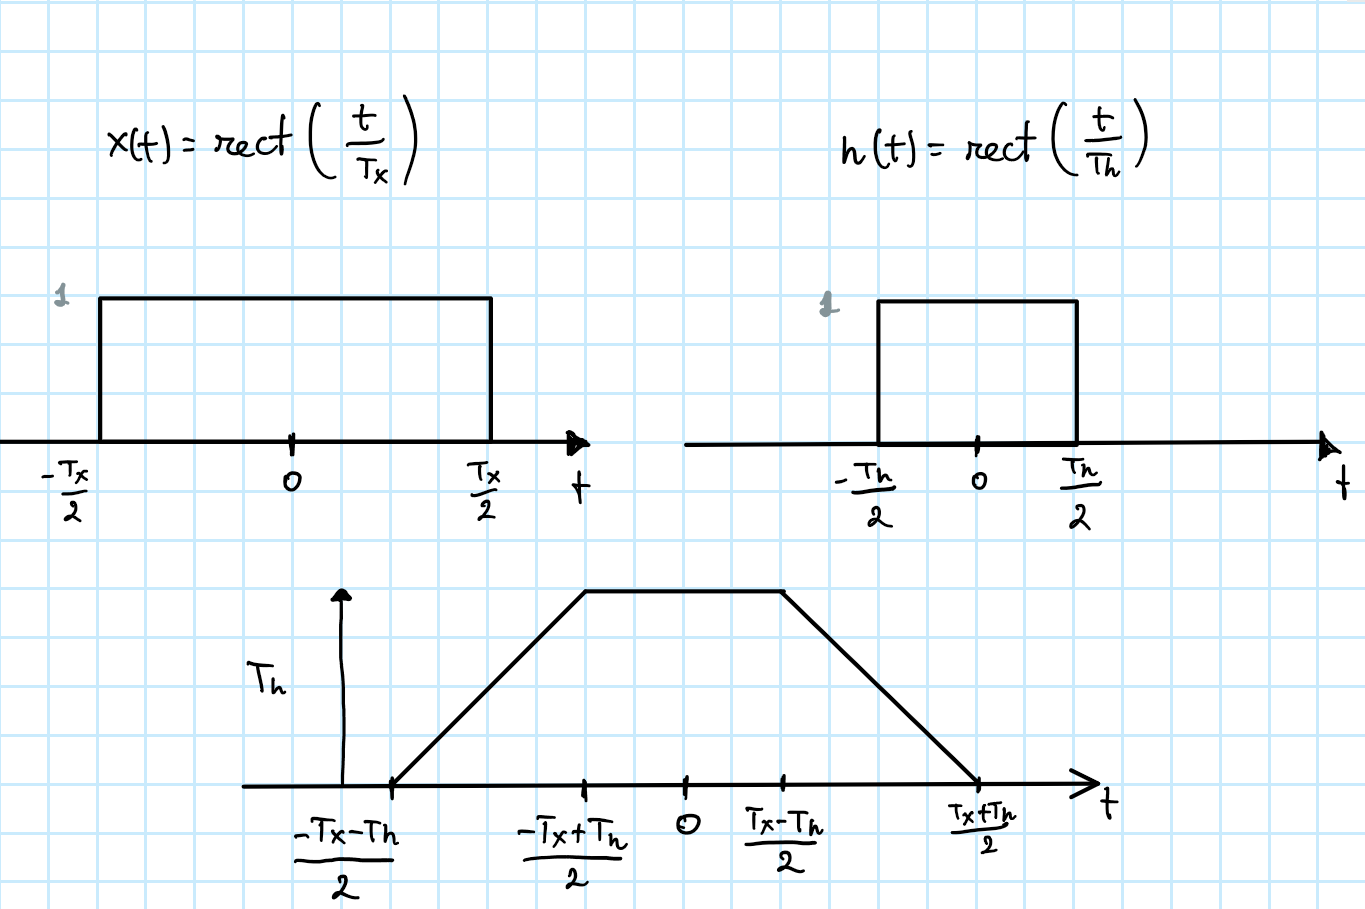
\includegraphics[scale=0.3]{convoluzione_rettangoli.png}
\end{center}

\end{enumerate}

\end{enumerate}

\newpage

\textit{\textbf{2. Trasformata di Fourier}}

\begin{enumerate}
\item \textit{Risposta in frequenza}
\\
Sia $h(t)$ la risposta all' impulso di un sistema LTI, allora la sua risposta in frequenza sarà

\begin{equation}
H(f)= \int_{- \infty}^{\infty} h(t) e^{-j2 \pi f t} dt
\end{equation}

\item \textit{Risposta di una sinusoide in ingresso}
\\
Consideriamo 
\[ Asin(2 \pi f_0 t)= \Im \left[ Ae^{-j2 \pi f_0 t} \right]\]
allora l'uscita $y(t)$ del sistema sarà data da
\begin{equation}
y(t)= \Im \left[ Ae^{-j2 \pi f_0 t} \int_{- \infty}^{\infty} h(t) e^{-j2 \pi f t} dt \right]= A |H(f)| sin( 2 \pi f_0 t + \angle H(f))
\end{equation}
\item \textit{Trasformate di Fourier utili}
\[\delta(t) \xrightarrow{\mathscr{F}}  1\]
\[1 \xrightarrow{\mathscr{F}}  \delta(f)\]
\[rect \left( \frac{t}{T} \right) \xrightarrow{\mathscr{F}}  T sinc(Tf)\]
\[Ae^{-j2 \pi f_0 t} \xrightarrow{\mathscr{F}} A \delta(f-f_0) \]
\[Asin(2 \pi f_0 t) \xrightarrow{\mathscr{F}}  \frac{Aj}{2} \delta(f+f_0) - \frac{Aj}{2} \delta(f-f_0)\]
\[Acos(2 \pi f_0 t) \xrightarrow{\mathscr{F}}  \frac{A}{2} \delta(f+f_0) + \frac{A}{2} \delta(f-f_0)\]

\item \textit{Il seno cardinale}
\\
Il seno cardinale è così definito
\begin{equation}
sinc(x)= \frac{sin(\pi x)}{\pi x}
\end{equation}
l' area di un seno cardinale vale
\begin{equation}
\int_{- \infty}^{\infty} Tsinc(Tf) df = T
\end{equation}
In oltre, il seno cardinale converge ad una delta di Dirac per $T \to \infty$
\end{enumerate}



\newpage









\begin{center}
\begin{Large}
\textbf{Formulario Probabilità e Statistica}
\end{Large}
\end{center}

\textbf{1. Definizioni basilari}

\begin{enumerate}

\item \textit{Probabilità del' unione } \\
la si usa nei casi in cui esca scritto "\textit{almeno}", in quel caso di fa riferimento ad una unione di insieme

\begin{equation}
P(A\cup B) = P(A)+P(B)-P(A, B) \ \ \Leftrightarrow \ \ A\cap B \neq \emptyset
\end{equation}

\item \textit{Probabilità condizionata } \\

\begin{equation}
P(A | B)= \frac{P(A, B)}{P(B)}
\end{equation}

\item \textit{probabilità congiunta} \\
La si usa nei casi in cui gli eventi accadono simultaneamente oppure siano in qualche modo dipendenti

\item \textit{Eventi indipendenti}
\\ Un evento è indipendente se

\begin{equation}
P(A | B)= P(A) \ \ \ \Leftrightarrow  \ \ \ P(A,B)=P(A)P(B)
\end{equation}

\item \textit{Teorema di Bayes}

\begin{equation}
P(B|A)=\frac{P(B) P(A|B)}{P(A)} 
\end{equation}

\item \textit{Probabilità totale}
\\ Siano dati $A$ e $B$ in modo tale che
\[B=\bigcup_{k} B_k  \ \ \ \ \bigcap_k (A\cap B_k)= \emptyset \]
allora vale il seguente risultato 

\begin{equation}
P(A \cap B)=\sum_k P(A \cap B_k)= \sum_k P(A | B_k)P(B_k)
\end{equation}

\end{enumerate}

\newpage 
\textbf{2. variabili casuali discrete e continue}
\\ 
\\

\textit{\textbf{2.1 Variabili casuali discrete}}
\\

Nel caso discreto si assegna ad una funzione $P_X (x_i)$ il valore di probabilità di ogni evento semplice $x_i$

\begin{enumerate}
\item \textit{Proprietà fondamentale}

\begin{equation}
\sum_{k=- \infty}^{\infty} P_X(x_k)=1
\end{equation}

\item \textit{funzione di ripartizione} \\ 
Nel caso discreto indica la probabilità che valori minori rispetto ad un evento $a$ possano essere risultato dell' esperimento

\begin{equation}
F_X (a)= P_X(X<a)= \sum_{k=-\infty}^{a} P_X(x_k)
\end{equation}

La funzione di ripartizione è \textit{monotona crescente} ed è tale per cui $F_X(- \infty)=0$ e $F_X(\infty)=1$

\item \textit{Probabilità multidimensionale (caso 2D)}\\
Se un esperimento dipende da più variabili casuali discrete $x_i$ e $y_j$ allora è possibile estendere a questo caso le due precedenti proprietà

\begin{enumerate}
\item
\begin{equation}
\sum_{i=- \infty}^{\infty} \sum_{j=- \infty}^{\infty} P_{XY}(x_i,y_i)=1
\end{equation}

\item \textit{Probabilità marginale}
\\ Indica la probabilità che si verifichi un evento se si fissa una delle variabili casuali discrete

\begin{equation}
P_{XY}(x_i)=\sum_{j=- \infty}^{\infty} P_{XY}(x_i,y_j)
\end{equation}

\item \textit{Probabilità condizionata}
\\ Applicando la definizione di probabilità condizionata

\begin{equation}
P(x_i | y_j)= \frac{P_{XY}(x_i,y_i)}{P_{XY}(y_j)}= \frac{P_{XY}(x_i,y_i)}{\sum_i P_{XY}(x_i,y_j)}
\end{equation}

\end{enumerate}

\end{enumerate}

\newpage

\textit{\textbf{2.2 Variabili casuali continue}}

\begin{enumerate}
\item \textit{Densità di probabilità}
\\ Nel caso di variabili casuali discrete non si può assegnare un valore di probabilità ad un punto. Si sceglie di assegnare una densità di probabilità

\begin{equation}
f_X(x)=\frac{P(x<X\leq x+dx)}{dx}
\end{equation}
\[0 \leq f_X(x) \leq 1 \] 

\item \textit{Probabilità}
\begin{equation}
P(a\leq X \leq B)= \int_a^b f_X(x) dx
\end{equation}
Vale la solita proprietà
\[ \int_{-\infty}^{\infty} f_X(x) dx=1\]

\item \textit{\textbf{Funzione di ripartizione}}
\begin{equation}
F_X(x)=P_X(X<x)=\int_{-\infty}^{x} f_X(\tilde{x})d \tilde{x}
\end{equation}
La funzione di ripartizione è una funzione integrale pertanto 

\begin{equation}
f_X(x)= \frac{dF_X(x)}{dx}
\end{equation}
Poiché la funzione di ripartizione è una primitiva di $f_X(x)$ vale anche

\begin{equation}
P_X(a<X<b)=\int_{a}^{b} f_X(x)d x= F_X(b)- F_X(a)
\end{equation}

\begin{enumerate}
\item \textit{\textbf{Percentile}} \\
Il percentile indica gli eventi che hanno al più un dato valore di probabilità. Ad esempio, il 10° percentile di un dato esperimento lo si può calcolare usando

\begin{equation}
F_X(x)=\frac{10}{100}
\end{equation}

\item \textit{\textbf{Mediana}} \\
La mediana è il 50° percentile e divide la densità di probabilità in due zone ad area pari a 0.5. L'evento $x \in X$ che rappresenta la mediana lo si calcola come

\begin{equation}
F_X(x)=\frac{1}{2}
\end{equation}

\end{enumerate}

\item \textit{Generalizzazione in più variabili}
Se si hanno più variabili casuali che concorrono nello stesso esperimento allora

\begin{equation}
f(x_1...x_n)=\frac{P(x_1<X_1\leq x_1+dx_1,...,x_n<X_n\leq x_n+dx_n)}{dx_1 ... dx_n}
\end{equation}
nelle due variabili invece

\begin{equation}
f_{XY}(x,y)=\frac{P(x<X\leq x+dx,y<Y\leq y+dy)}{dx dy}
\end{equation}

Assegnato il dovuto dominio di integrazione, la probabilità sarà

\begin{equation}
P= \iint_{\Omega} f_{XY}(x,y) dx dy
\end{equation}

è possibile definire la \textit{probabilità marginale}

\begin{equation}
P(x_i)= \int_{-\infty}^{\infty} f(x_i,y)dy \ \ \ x_i \in \R
\end{equation}

La \textit{densità di probabilità condizionata} sarà invece

\begin{equation}
f(x|y)=\frac{f(x,y)}{f(y)}=\frac{P(x<X\leq x+dx,y<Y\leq y+dy)}{dx dy \frac{P(y<Y\leq y+dy)}{dy}}
\end{equation}
Si osservi che tecnicamente i $dy$ si semplificano. Una \textbf{tipologia di esercizi} (\textit{Bellini - 1.14}) usano questo risultato.
\\
\textit{"Sia $f(x)=1-\frac{x}{2}$, calcolare $f(x|X> 1)$".}
Usando la formula precedente si ha
\[
f(x|X>1)=\frac{P(x<X\leq x+dx,X>1)}{dx P(X>1)}
\]
Sappiamo calcolarci $P(X>1)$
\[
P(X>1)=\int_{-\infty}^{\infty} 1- \frac{x}{2}dx=\frac{1}{4}
\]
\\
Dunque
\[
f(x|X>1)=\frac{P(x<X\leq x+dx,X>1)}{dx \cdot \frac{1}{4}}= 4f(x) \ \ \ \ \ se \ \ 1<x<2
\]


\item \textit{Condizione di indipendenza statistica}
\\
La condizione di indipendenza statistica di due variabili casuali $X,Y$ risulta essere data da
 \begin{equation}
 f_{X,Y}(x,y)=f_X(x)f_Y(y)
 \end{equation}
 Il grafico di questa funzione in 2 variabili conserva la \textit{shape della $f_Y(y)$} scorrendo le $x$, mentre conserva la \textit{shape della $f_X(x)$} scorrendo le $y$
\end{enumerate}

\newpage

\textit{\textbf{2.3 Trasformazioni di variabili casuali}}

\begin{enumerate}
\item \textit{Caso discreto ed eventi $X$ e $Y$ indipendenti}\\
Sia $Z=g \left( X,Y \right)$  una trasformazione di variabili casuali discrete. Si procede in questo modo
\begin{enumerate}
\item Si definisce la 
\[ Z=g \left( X,Y \right) \]
\item Si costruisce lo spazio degli eventi congiunti $(x_i,y_i)$.
\\
\end{enumerate}
La probabilità totale dell' evento Z sarà data da
\begin{equation}
P(Z)= \sum_i \sum_k P(x_i,y_i) \delta(g(x_i,y_i)-z)
\end{equation}

\item \textit{Caso continuo per $g: \R \to \R$ monotona}
\\
Supponiamo $Y=g(X)$,con $g: \R \to \R$ monotona crescente o decrescente. Se è nota a priori la \textit{ddp} dell' evento $X$, allora è possibile ricavare anche la stessa (e anche la ripartizione \textit{ddp} scritta con l'evento $Y$.
\\
Detta 
\[X= g_I (Y) \]
la funzione inversa di $g$, allora:

\begin{enumerate}
\item nel caso si vogliano trovare le \textit{funzioni di ripartizione}, se \textit{$g(X)$ è monotona crescente} si ha
\begin{equation}
F_Y (y)= F_X(g_I(y))
\end{equation}
Se invece la funzione $g$ è \textit{monotona decrescente}
\begin{equation}
F_Y(y)=1-F_X(g_I(y))
\end{equation}

\item se invece si vuole la \textit{ddp} riscritta con l'evento $y$ la formula generale è la seguente

\begin{equation}
f_Y(y)=\frac{f_X(g_I(y))}{|g'(g_I(y))|}
\end{equation}
quindi assicurarsi sempre di avere
\begin{enumerate}
\item la $f_X$ (solitamente è un dato) e la $Y=g(X)$
\item la derivata di $g$, cioè $g'(x)$
\item la funzione inversa $g_I(y)$ che poi dovrà essere sostituita.
\end{enumerate}

\item Esiste una formula più comoda data da Manzoni

\begin{equation}
F_Y (y)=P(Y\leq y)= P( g(x) \leq y) = P(x \leq g_I(y))= F_X (g_I(y))
\end{equation}
Derivando si ottiene
\begin{equation}
f_Y(y)= \frac{\partial F_Y}{\partial y}= f_X(g_I(y)) \left| \frac{\partial}{\partial y} g_I(y) \right|
\end{equation}
\end{enumerate}

\item \textit{Caso continuo per $g: \R \to \R$} \textit{generica} \\
Se una funzione $g$ non è biunivoca, ma è localmente invertibile, per calcolare la $f_Y(y)$ è necessario dividere il problema e sommare tutti i risultati che si ottengono. In generale, detto l'$i$-esimo intervallo di locale monotonia, si ha

\begin{equation}
f_Y(y)=\sum_{i}\frac{f_X(g_I(y))}{|g'(g_I(y))|}
\end{equation}

\item \textit{Caso $g: \R^n \to \R$ solo somme di v.c.}
\\
Sia $Z=f(X_1,...,X_n)$, allora
\begin{equation}
f_Z(z)=x_1(z)*x_2(z)*...*x_n(z)
\end{equation}
\end{enumerate}

\newpage

\textbf{Distribuzioni}

\begin{enumerate}

\item \textit{Distribuzione esponenziale}

La distribuzione esponenziale è una distribuzione del tipo

\begin{equation}
f_T(t)=\frac{1}{\tau} e^{-\frac{t}{\tau}}
\end{equation}

\begin{center}
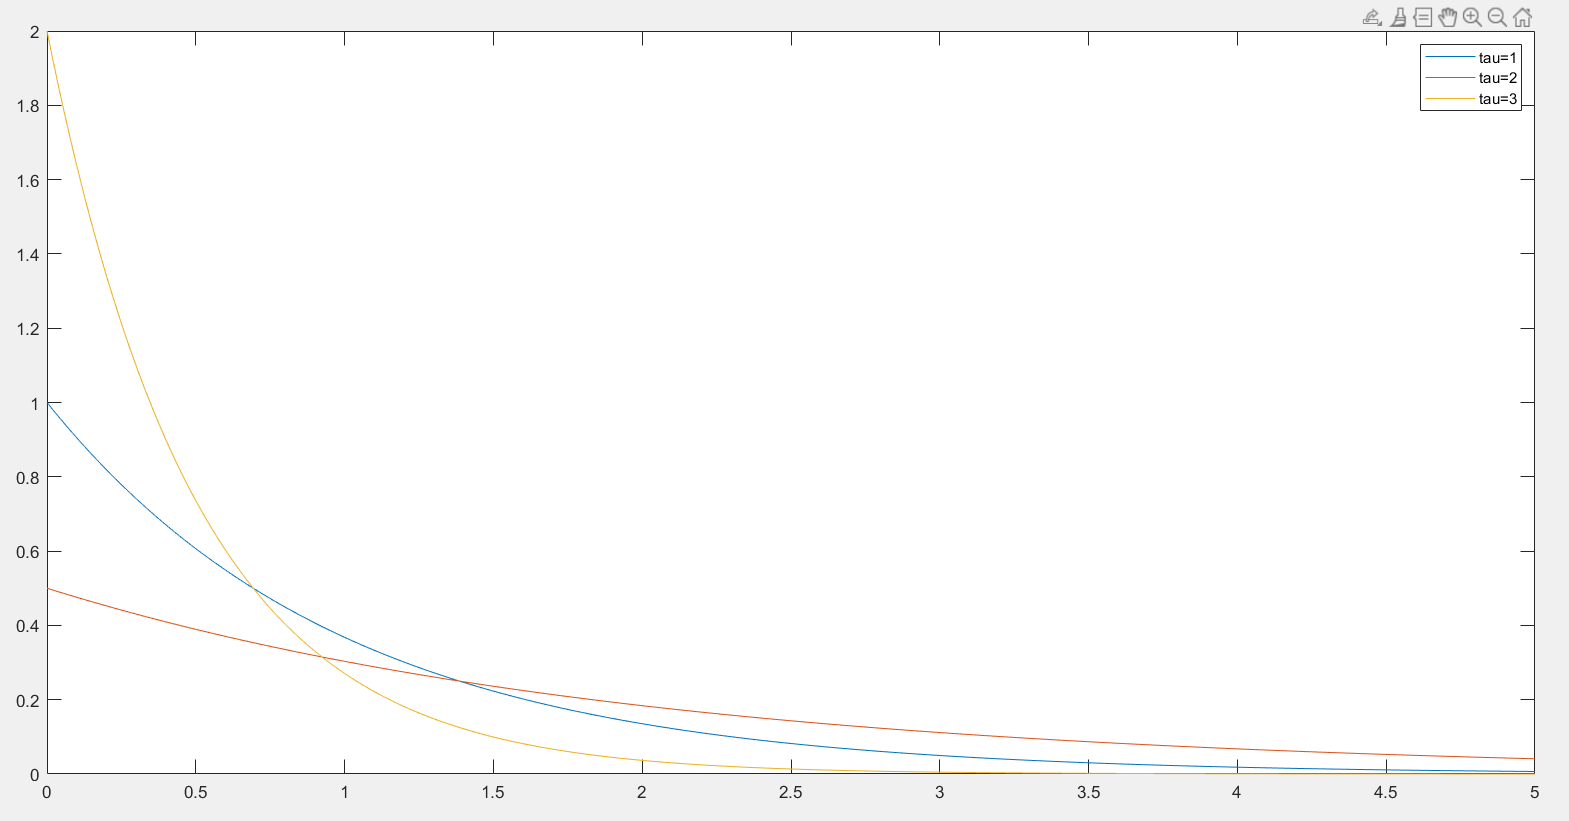
\includegraphics[scale=0.18]{distribuzione_esponenziale.png}
\end{center}

\item \textit{\textbf{Distribuzione gaussiana}}
\\
Assegnati i valori $\mu$ e $\sigma$ detti rispettivamente \textit{media} e \textit{varianza}, la gaussiana è assegnata da
     
\begin{equation}
N(\mu,\sigma^2)  = \frac{1}{\sqrt{2 \pi} \sigma} e^{- \frac{(x- \mu)^2}{2 \sigma^2}}
\end{equation}
\begin{center}
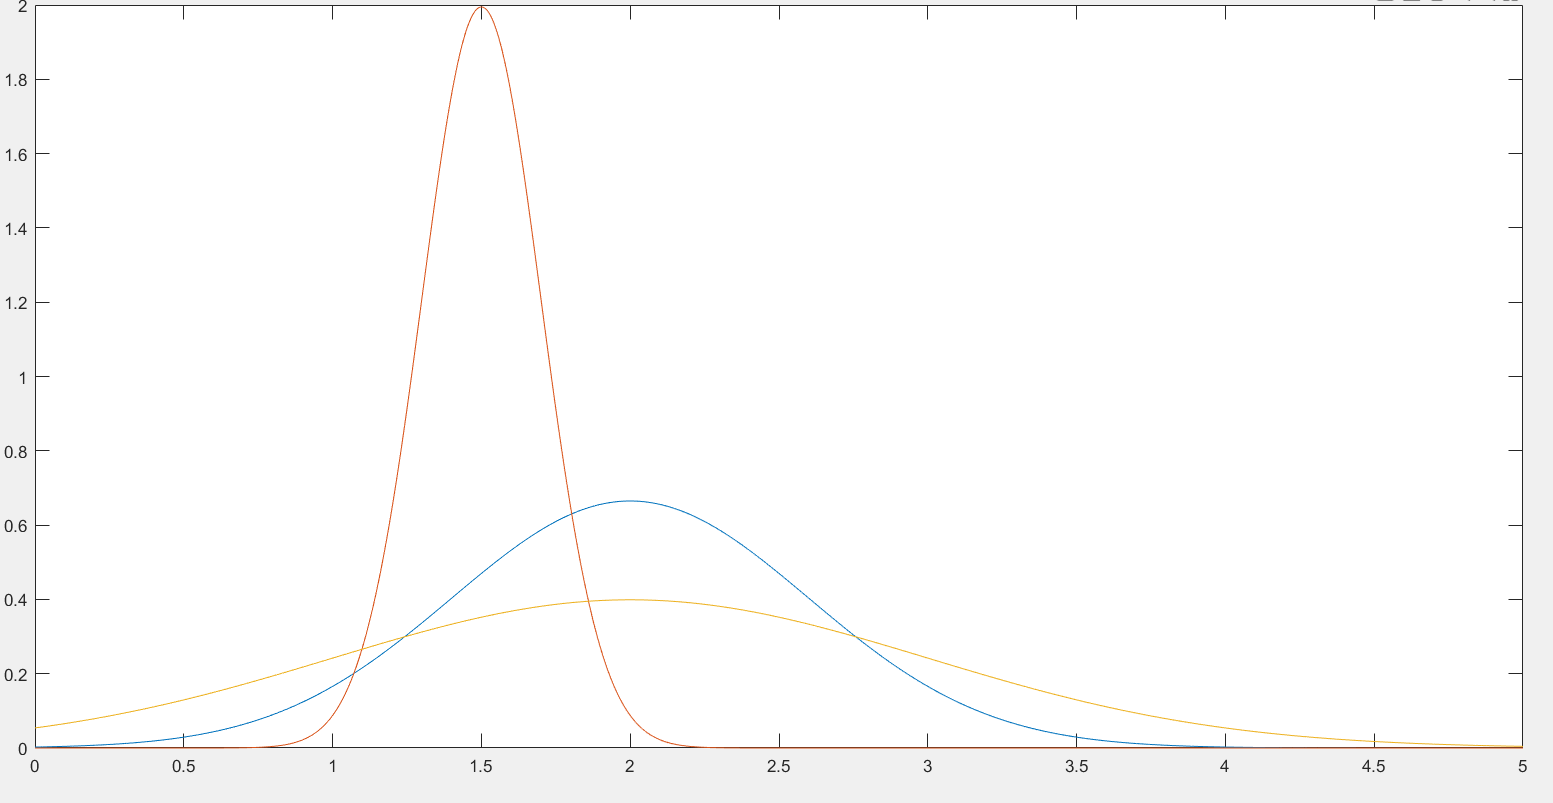
\includegraphics[scale=0.2]{gaussiane.png}

\end{center}

La gaussiana ha anche definita la funzione $Q$
\[
 Q(x_0)= 1-F(x_0) = \int_{x_0}^{\infty} N(\mu,\sigma^2) dx
\]
In oltre vanno considerati gli \textbf{intervalli di confidenza} che sono intervalli simmetrici centrati nell' asse di simmetria della gaussiana ($x= \mu$). Scostamenti di $  \pm \sigma$ coprono il $70 \%$ di probabilità degli eventi, mentre $ \pm 2 \sigma$ copre il $95 \%$ e $ \pm 3 \sigma $ copre il $99,7 \%$ .

\item \textit{\textbf{Funzione binomiale}}
\\
La funzione binomiale si chiede: \textit{Date $N$ prove ripetute (lanci di dadi o monete, tentativi...) e data la probabilità $p$ che un evento possa accadere ad ogni singola prova, qual è la probabilità che esso si verifichi $k$ volte?} 
\begin{equation}
P_N(k)= \binom{N}{k} p^k (1-p)^{N-K}
\end{equation}
Per $N \to \infty$ la distribuzione binomiale (che è discreta) tende ad una gaussiana che possiede
\[
\mu= pN
\]
\[
\sigma= \sqrt{Np(1-p)}
\]

\begin{center}
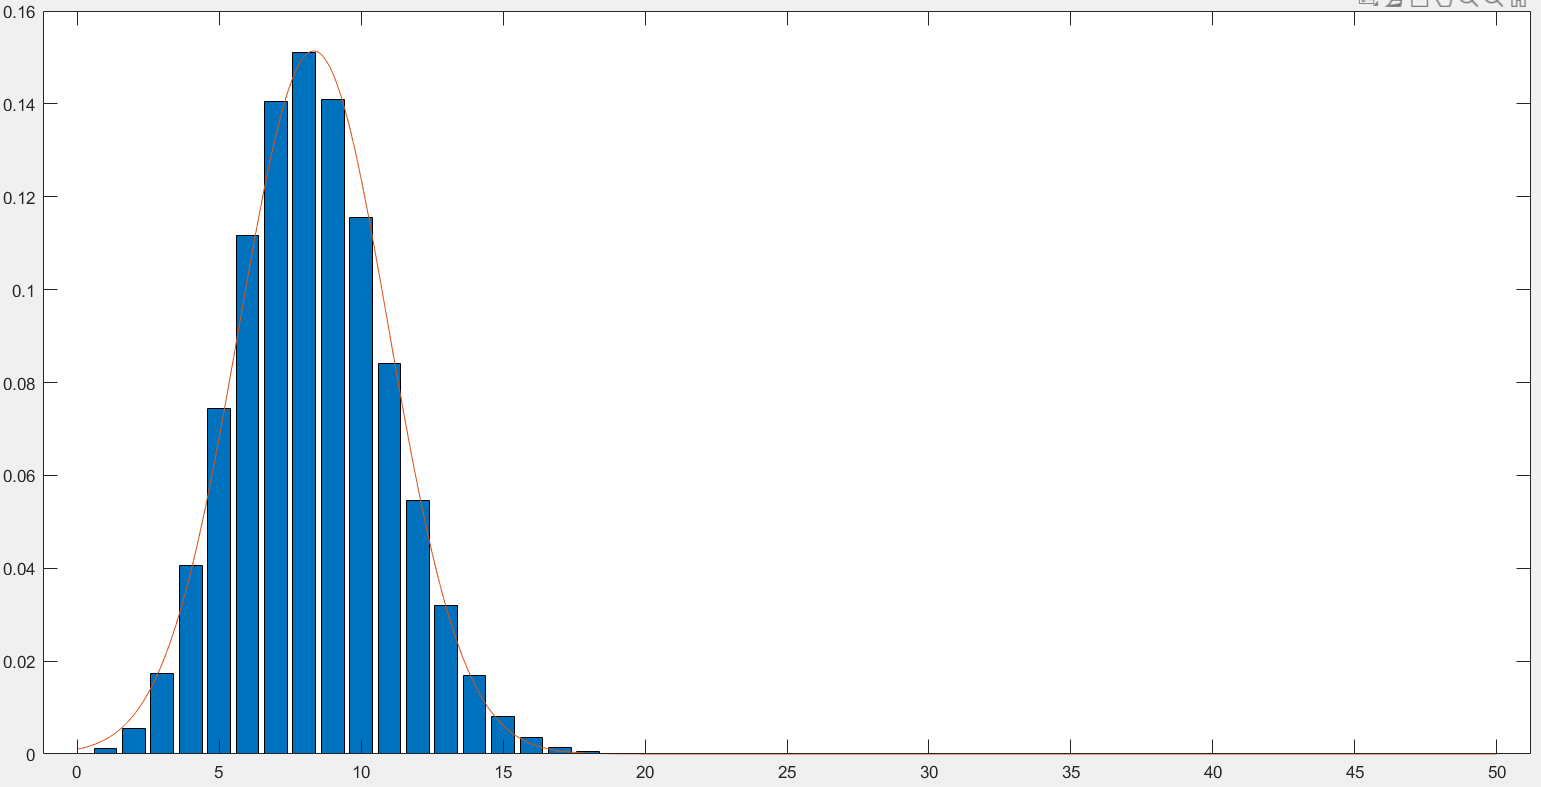
\includegraphics[scale=0.2]{binomiale}
\\

\begin{small}
plot della binomiale con $N=50$ e $p=\frac{1}{6}$
\end{small}
\end{center}
Normalizzare la gaussiana per $N$ fornisce la \textbf{frequenza relativa}, cioè una distribuzione che segna gli intervalli di confidenza con cui si percepisce $p$.
\begin{equation}
\eta= \frac{K}{N}
\end{equation}
Anche la frequenza relativa tende ad una distribuzione gaussiana con 
\[
\mu= p
\]
\[
\sigma= \frac{\sqrt{p(1-p)}}{\sqrt{N}}
\]
\begin{center}
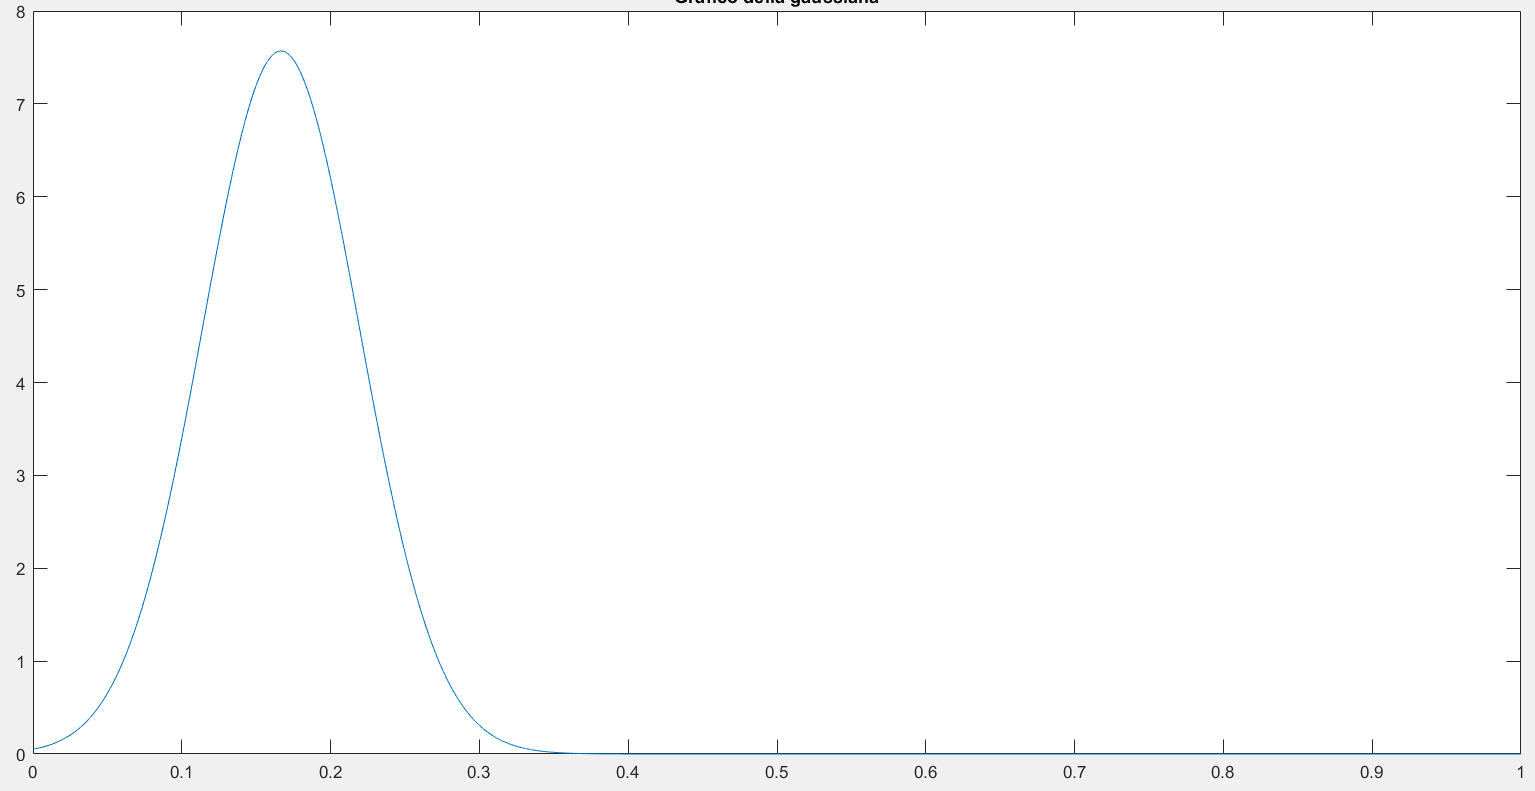
\includegraphics[scale=0.2]{frequenza_relativa.png}
\end{center}
Per ultimo definiamo \textit{incertezza relativa}  come la quantità che mi rivela di quanto sbaglio la misura di probabilità per ogni singolo evento.
\begin{equation}
\varepsilon=\frac{\sigma}{p}
\end{equation}
per piccole probabilità l'espressione diventa
\[
\varepsilon= \frac{1}{\sqrt{Np}}
\]

\end{enumerate}


\end{document}